\documentclass[../TDAM3.tex]{subfiles}%

\begin{document}
\section{Structure d'un alliage du titane}
\enonce{%
	\begin{isd}[righthand ratio=.4]
		L'alliage le plus utilisé dans l'industrie aéronautique a pour formule brute
		\ce{Al_xNi_yTi_z}. Le titane y est présent sous forme $\beta$~: son système
		cristallographique est le CFC. Les atomes d'aluminium occupent la totalité des
		sites octaédriques, et ceux de nickel occupent tous les sites tétraédriques. Le
		paramètre de la maille ainsi formée vaut $a = \SI{589}{pm}$.
		\tcblower
		\begin{center}
			\captionof{table}{Données par atome}
			\begin{tabular}{ccc}
				\toprule
				Atome   & $R\ind{atome}$ (\si{pm}) & $M$ (\si{g.mol^{-1}})
				\\\midrule
				\ce{Ti} & \num{147}                & \num{47.90}
				\\
				\ce{Al} & \num{143}                & \num{26.98}
				\\
				\ce{Ni} & \num{124}                & \num{58.70}
				\\\bottomrule
			\end{tabular}
		\end{center}
	\end{isd}
}%
\QR{%
	Représenter la maille cubique en perspective.
}{%
	Voir figure.
	\begin{figure}[h]
		\centering
		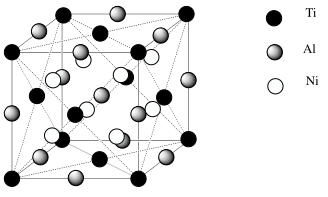
\includegraphics[scale=.8]{titane_alliage}
		\caption{Maille élémentaire de l'alliage. Les couleurs sont indiquées dans
			la légende.}
		\label{fig:titall}
	\end{figure}
}%

\QR{%
	Déterminer la formule de l'alliage.
}{%
	Dans une structure CFC, il y a autant de sites O que d'atomes par
	maille, et deux fois plus de sites T que d'atomes par maille. Ainsi, la
	formule de l'alliage est~:
	\[
		\boxed{\ce{AlNi_2Ti}}
	\]
}%

\QR{%
	Calculer l'habitabilité des sites T et O.
}{%
	L'arête est de longueur $a = \SI{589}{pm}$. On trouve les sites O au
	milieu de l'arête. La condition de tangence s'écrit donc~:
	\[
		a = 2 (r_{\ce{Ti}} + r_{\mathrm{O}})
		\qqdonc
		\boxed{r_{\mathrm{O}} = \frac{a}{2} - r_{\ce{Ti}} = \SI{147.5}{pm}}
	\]
	ce qui est effectivement suffisant pour l'aluminium. Le site T est sur la
	grande diagonale des petits cubes d'arête $a/2$, d'où
	\[
		a \frac{\sqrt{3}}{2} = r_{\ce{Ti}} + 2r_{\mathrm{T}} + r_{\ce{Al}}
		\qqdonc
		\boxed{r_{\mathrm{T}} = \frac{1}{2} \left( a \frac{\sqrt{3}}{2} -
			r_{\ce{Ti}} - r_{\ce{Al}} \right) = \SI{110}{pm}}
	\]
	ce qui est un peu faible pour l'atome de nickel.
}%

\QR{%
	Calculer la compacité et la masse volumique de cet alliage.
}{%
	$C$ est le rapport volume occupé/volume de la maille~:
	\[
		C = \frac{4\times \frac{4}{3}\pi r_{\ce{Ti}}^{3} + 4\times \frac{4}{3}\pi
			r_{\ce{Al}}^{3} + 8\times \frac{4}{3}\pi r_{\ce{Ni}}^{3}}{a^3}
		= \frac{16\pi}{3a^3} \left( r_{\ce{Ti}}^{3} + r_{\ce{Al}}^{3} +
		r_{\ce{Ni}}^{3} \right) = \num{0.813}
	\]
	et pour la masse volumique~:
	\[
		\rho = \frac{4 (M_{\ce{Ti}} + M_{\ce{Al}} + 2M_{\ce{Ni}})}{\Nc_Aa^3}
		= \SI{6250}{kg.m ^{-3}}
	\]
}%

\QR{%
	Comparer les valeurs trouvées précédemment aux caractéristiques moyennes
	d'un acier courant~: $\rho_a = \SI{7800}{kg.m ^{-3}}$, de compacité
	$C\ind{acier} = \num{0.70}$. À qualités mécaniques équivalentes,
	expliquer
	en quoi l'alliage de titane présente de l'intérêt.
}{%
	L'alliage est utilisé car notablement moins dens, donc la masse des
	appareils s'en trouve réduite.
}%

\end{document}
